\documentclass[10pt]{article}
\usepackage{caption}
\usepackage{multirow}
\usepackage{amsfonts}
\usepackage{amsmath}
\usepackage{amssymb}

\usepackage{tikz}
\usepackage{tkz-euclide}
\usetikzlibrary{shapes, backgrounds, calc}
\usetkzobj{all}

\usepackage{hyperref}
\hypersetup{
	colorlinks = true
}

\begin{document}
	\tableofcontents
	\pagebreak

	\section{Review of Propositional Logic}
	\begin{description}
		\item[Task:] Recall enough propositional logic to see how it matches up with set theory.
		\item[Definition:] A \underline{proposition} is any declarative sentence that is either true or false.
	\end{description}
	
	\subsection{Connectives}
	\centerline {
		\begin{tabular}{cccc}
			\multicolumn{3}{c}{\underline{Connectives}} & \multicolumn{1}{c}{\underline{Notation in Maths}} \\
			and & $\land$ \\
			or & $\lor$ & "Inclusive or"\\
			not & $\lnot$ & Sometimes denoted $\sim$\\
			implies & $\to$ & if/then; called implication & $\Rightarrow$\\
			if and only if & $\leftrightarrow$ & Called equivalence & $\Leftrightarrow$\\
		\end{tabular}
	}
	
	\subsubsection{Truth Table of the Connectives}
	Let P, Q be propositions:\\

	\centerline{	
		\begin{tabular}{|c|c|c|}
			\cline{1-3}
			P & Q & P$\land$Q \\ \cline{1-3}
			F & F & F \\ \cline{1-3}
			F & T & F \\ \cline{1-3}
			T & F & F \\ \cline{1-3}
			T & T & T \\ \cline{1-3}
		\end{tabular}
		\quad
		\begin{tabular}{|c|c|c|}
			\cline{1-3}
			P & Q & P$\lor$Q \\ \cline{1-3}
			F & F & F \\ \cline{1-3}
			F & T & T \\ \cline{1-3}
			T & F & T \\ \cline{1-3}
			T & T & T \\ \cline{1-3}
		\end{tabular}
		\quad
		\begin{tabular}{|c|c|}
			\cline{1-2}
			P & $\lnot$P \\ \cline{1-2}
			F & T \\ \cline{1-2}
			T & F \\ \cline{1-2}
		\end{tabular}
		\quad
		\begin{tabular}{|c|c|c|}
			\cline{1-3}
			P & Q & P$\to$Q \\ \cline{1-3}
			F & F & T \\ \cline{1-3}
			F & T & T \\ \cline{1-3}
			T & F & F \\ \cline{1-3}
			T & T & T \\ \cline{1-3}
		\end{tabular}
		\quad
		\begin{tabular}{|c|c|c|}
			\cline{1-3}
			P & Q & P$\leftrightarrow$Q \\ \cline{1-3}
			F & F & T \\ \cline{1-3}
			F & T & F \\ \cline{1-3}
			T & F & F \\ \cline{1-3}
			T & T & T \\ \cline{1-3}
		\end{tabular}
	}
	
	\subsubsection*{Priority of the Connectives}
	\textbf{Highest to Lowest:} $\lnot, \land, \lor, \rightarrow, \leftrightarrow$
	
	\subsection{Important Tautologies}
	\begin{tabular}{rcll}
		$(P \rightarrow Q)$ & $\leftrightarrow$ & $(\lnot P \lor Q)$ \\
		$(P \leftrightarrow Q)$ & $\leftrightarrow$ & $[(P \rightarrow Q) \land (Q \rightarrow P)]$ \\
		$\lnot(P \land Q)$ & $\leftrightarrow$ & $(\lnot P \lor \lnot Q)$ & \multirow{2}{4cm}{\LARGE\} \normalsize De Morgan Laws} \\
		$\lnot(P \lor Q)$ & $\leftrightarrow$ & $(\lnot P \land \lnot Q)$ \\
	\end{tabular}
	~\\~\\~\\
	As a result, $\lnot$ and $\lor$ together can be used to represent all of $\lnot, \land, \lor, \rightarrow, \leftrightarrow$.
	
	\begin{description}
		\item[Less obvious:] One connective called the sheffer stroke P$\mid$Q (which stands for "not both P and Q" or "P nand Q") can be used to represent all of $\lnot$, $\land$, $\lor$, $\rightarrow$, $\leftrightarrow$ since $\lnot$P $\leftrightarrow$ P$\mid$P and P $\lor$ Q $\leftrightarrow$ (P$\mid$P) $\mid$ (Q$\mid$Q).
		\item[Recall] is P$\rightarrow$Q is a given implication, Q$\rightarrow$P is called the \underline{converse} or P$\rightarrow$Q. $\lnot$Q $\rightarrow$ $\lnot$P.
	\end{description}
	
	\subsection{Indirect Arguments/Proofs by Contradiction/Reductio as absurdum}
	Based on the tautology (P$\rightarrow$Q) $\leftrightarrow$ ($\lnot$Q $\rightarrow$ $\lnot$P)
	
	\begin{description}
		\item[Example:] Famous argument that $\sqrt{2}$ is irrational.
		\item[Proof:]
		\item \textbf{Suppose} $\sqrt{2}$ is rational, then it can be expressed is fraction form $\frac{a}{b}$. Let us \textbf{assume} that our fraction is in the lowest term, \textbf{i.e.} their only common divisor is 1.
		\item Then, \[\sqrt{2}=\frac{a}{b}\]
		\item Squaring both sides, we have \[2=\frac{a^2}{b^2}\]
		\item Multiplying both sides by $B^2$ yields \[2b^2=a^2\]
		\item Since $a^2b^2$, we can conclude that $a^2$ is even because whatever the value of $b^2$ has to be multiplied by 2. Is $a^2$ is even, then $a$ is also even. Since $a$ is even, no matter what the value of $a$ is, we can always find an integer that if we divide $a$ by 2, it is equal to that integer. If we let that integer be $k$, then $\frac{a}{b}=k$ which means that $a=2k$.
		\item Substituting the value of $2k$ to $a$, we have $2b^2=(2k)^2$ which means that $2b^2=4k^2$. dividing both sides by 2 we have $b^2=2k^2$. That means that the value $b^2$ is even, since whatever the value of $k$ you have to multiply it by 2. Again, is $b^2$ is even, then $b$ is even.
		\item This implies that both $a$ and $b$ are even, which means that both the numerator and the denominator of our fraction are divisible by 2. This contradicts our \textbf{assumption} that $\frac{a}{b}$ has no common divisor except 1. Since we found a contradiction, our assumption is, therefore, false. Hence the theorem is true.
		\item \textbf{qed}
	\end{description}
	
	\section{Predicate logic and Quantifiers}
	\begin{description}
		\item[Task:] Understand enough predicate logic to make sense of quantified statements.
		\item In predicate logic, propositions depend on variable x, y, x, so their truth value may chance depending on which values these variables assume: $P(x), Q(x, y), R(x, y, z)$
	\end{description}
	
	\subsection{Introduce quantifiers}
	\subsubsection{$\exists$ existential quantifier}
	\begin{description}
		\item[Syntax:] $\exists xP(x)$
		\item[Definition:] $\exists xP(x)$ is true if $P(x)$ is true or some value of $x$; it is false otherwise.
	\end{description}
	
	\subsubsection{$\forall$ universal quantifier}
	\begin{description}
		\item[Syntax:] $\forall xP(x)$
		\item[Definition:] $\forall xP(x)$ is true if $P(x)$ is true for all allowable values of $x$. It is false otherwise.
	\end{description}
	
	\subsubsection{$\exists!$ for one and only one}
	\begin{description}
		\item[Syntax:] $\exists! xP(x)$
		\item[Definition:] $\exists! xP(x)$ is true if $P(x)$ is true for exactly one value of $x$ and false for all often values of $x$; otherwise, $\exists! xP(x)$ is false.
	\end{description}
	
	\subsection{Alternation of Quantifiers}
	\begin{tabular}{lr}
		$\forall x\exists y\forall z$ & $P(x, y, z)$ \\
	\end{tabular}
	~\\
	\textbf{NB:} The order \underline{cannot} be exchanged as it might modify the truth values of the statement (think of examples with two quantifiers).
	
	\subsection{Negation of Quantifiers}
	\begin{tabular}{rcl}
		$\lnot(\exists xP(x))$ & $\leftrightarrow$ & $\forall x\lnot P(x)$ \\
		$\lnot(\forall xP(x))$ & $\leftrightarrow$ & $\exists x\lnot P(x)$ \\
	\end{tabular}
	
	\section{Set Theory}
	\begin{description}
		\item[Task:] Understand enough set theory to make sense of other mathematical objects in abstract algebra, graph theory, etc. Set theory started around 1870's $\rightarrow$ late development in mathematics but now taught early in one's maths education due to Bourbaki school.
		\item[Definition:] A set is a collection of objects. $x\in A$ means the element $X$ is in the set $A$ (\textbf{i.e.} belongs to $A$).
		\item[Examples:] 
		\begin{enumerate}
			\item[]
			\item All students in a class.
			\item $\mathbb{N}$ the set of natural numbers starting at 0.
			\begin{enumerate}
				\item [$\mathbb{N}$] is defined via the following two axioms:
				\item 0 $\in \mathbb{N}$
				\item if $x \in \mathbb{N}$ then $x+1 \in \mathbb{N}$ ($x \in \mathbb{N} \rightarrow X+A \in \mathbb{N}$)
			\end{enumerate}
			\item $\mathbb{R}$ set of real numbers also introduced axiomatically
			\begin{enumerate}
				\item[$\mathbb{R}$] the set of real numbers.
				\item Additive closure: $\forall x, y \exists z (x+y=z)$
				\item Multiplicative closure: $\forall x, y, \exists z (x \times y=z)$
				\item Additive associativity: $x+(y+z)=(x+y)+z$
				\item Multiplicative associativity: $x \times (y \times z) = (x \times y) \times z$
				\item Additive commutativity: $x+y=y+x$
				\item Multiplicative commutativity: $x \times y = y \times x$
				\item Distributivity: $x \times (y+z) = (x \times y) + (x \times z)$ and $(y+z) \times x = (y \times x) + (z \times x)$
				\item Additive identity: There is a number, denoted 0, such that or all $x, x+0=x$
				\item Multiplicative identity: There is a number, denoted 1, such that for all $x, x \times 1 = 1 \times x = x$
				\item Additive inverses: For every $x$ there is a number, denoted $-x$, such that $x+(-x)=0$
				\item Multiplicative inverses: For every nonzero $x$ there is a number, denoted $x$, such that $x \times x^{-1} = x^{-1} \times x = 1$
				\item $0 \neq 1$
				\item Irreflexivity of $<: \sim (x<x)$
				\item Transitivity of <: If $x<y$ and $y<z$, then $x<z$
				\item Trichotomy: Either $x<y, y<x,$ or $x=y$
				\item If $x<y$, then $x+y<y+z$
				\item If $x<y$ and $0<z$, then $x \times z < y \times z$ and $z \times x < z \times y$
				\item Completeness: If a nonempty set of real numbers has an upper bound, then it has a \textit{least} upper bound.
			\end{enumerate}
			\item $\emptyset$ is the empty set (The set with no elements).
		\end{enumerate}
		\item[Definition:] Let A, B be sets. A=b if and only if all elements of A are elements of B and all elements of B are elements of A,\\i.e. $A=b \leftrightarrow [\forall x (x \in A \rightarrow x \in B)] \cap [\forall y (y \in B \rightarrow y \in A)]$
	\end{description}
		
	\subsection{Two Ways to Describe Sets}
	\begin{enumerate}
		\item The enumeration/roster method: list all elements of the set.\\ \textbf{NB:} order is \underline{irrelevant}.\\ $A=\{0, 1, 2, 3, 4, 5\}=\{5, 0, 2, 3, 1, 4\}$
		\item The formulaic/set builder method: give a formula that generates all elements of the set.\\ $A=\{x \in \mathbb{N} \mid 0 \leq 5 \land x \leq 5\} = \{0, 1, 2, 3, 4, 5\} = \{x \in \mathbb{N} : 0 \leq x \land x \leq 5 \}$
	\end{enumerate}
	Using $\mathbb{N}$ and the set-builder method, we can define:
		
	$\mathbb{Z} = \{m-n \mid \forall m, n \in \mathbb{N} \}$
		
	\hspace{5mm} $n=0$ in any natural numbers $\Rightarrow$ we generate all of $\mathbb{N}$
		
	\hspace{5mm} $m=0$ in any natural number $\Rightarrow$ we generator all negative integers
		
	$\mathbb{Q} = \{\frac{p}{q} \mid p, q \in \mathbb{Z} \land q \neq 0 \}$
	\begin{description}
		\item[Definition:] A set $A$ is called finite if it has a finite number of elements; otherwise it is called infinite.
	\end{description}
		
	\section{Set Operations}
	\begin{description}
		\item[Task:] Understand how to represent sets by Venn diagrams. Understand set union, intersection, complement and difference.
		\item[Definition:] Let $A, B$ be sets. $A$ is a \underline{subset} of $B$. If all elements of $A$ are elements of $B$, \textbf{i.e.} $\forall x(x \in A \rightarrow x \in B)$. We denote that $A$ is a subset of $B$ by $A \subseteq B$
		\item[Example:] $\mathbb{N} \subseteq \mathbb{Z}$
		\item[Definition:] Let $A, B$ be sets. $A$ is a \underline{proper} subset of $B$ if $A \subseteq B \land A \neq B$, \textbf{i.e.} $A \subseteq B \land \exists x \in B s.t. x \notin A$. \\ A proper subset is always a subset, but a subset is not always a proper subset.
		\item[Notation:] $A \subset B$
		\item[Example:] $\mathbb{N} \subset \mathbb{Z}$ since $\exists -1 \in \mathbb{N}$ \\ \textbf{NB:} $\forall A$ a set $\emptyset \subseteq A$
		\item[Recall:] $B \subseteq C$ means $\forall x(x \in B \rightarrow x \in C)$, but $\emptyset$ has no elements so in $\emptyset \subseteq A$ the quantifier $\forall$ operates on a domain with no elements. Clearly, we need to give meaning to $\exists$ and $\forall$ on empty sets.
	\end{description}
	
	\begin{tabular}{cc}
		\underline{Boolean Convention} \\
		$\forall$ is true on the empty set & \multirow{2}{6cm}{\LARGE\} \normalsize Consistent with common sense} \\
		$\exists$ is false on the empty set
	\end{tabular}
	
	\begin{description}
		\item[Definition:] Let $A, B$ be two sets. The \underline{union} $A \cup B = \{x \mid x \in A \lor x \in B \}$
		\item[Definition:] Let $A, B$ be two sets. The \underline{intersection} $A \cap B = \{x \mid x \in A \land x \in B \}$
		\item[Definition:] Let $A, B$ be sets. $A$ and $B$ are called \underline{disjoint} is $A \cap B = \emptyset$
		\item[Definition] Let $A, B$ be two sets. $A-B = A \backslash B = \{a \mid x \in A \land x \notin B \}$
		\item[Examples:]
		\begin{tabular}{ll}
			$A = \{1, 2, 5\}$ & $B = \{1, 3, 6\}$ \\
			$A \cup B = \{1, 2, 3, 5, 6\}$ & $A \cap B = \{1\}$ \\
			$A \backslash B = \{2, 5\}$ & $B \backslash A = \{3, 6\}$ \\
		\end{tabular}
		\item[Definition:] Let $A, U$ be sets s.t. $A \subseteq U$. The \underline{complement} of $A$ in $U$ = $U \backslash A = A^C = \{x \mid x \in U \land x \notin A \}$
		\item[Remark:] The notation $A^C$ is unambiguous only if the universe U is clearly defined or understood.
	\end{description}
	
	\subsection{Venn Diagrams}
	Schematic representation of set operations. \\

	\begin{figure}[h]
		\centering
		\def \setu{(0, 0)rectangle(4.5, 3)}
		\def \seta{(1.5, 1.5)circle(1)}
		\def \setb{(3, 1.5)circle(1)}
		\begin{tikzpicture}
			
			\begin{scope}
				\draw \seta node{$A$};
				\draw \setb node{$B$};
				\draw \setu;
			\end{scope}
			
			\begin{scope}[shift={(5cm, 0cm)}, even odd rule]
				\draw \seta node{$A$};
				\draw \setb node{$B$};
				\draw \setu (2.25, -0.5) node{$A^C$};
				\clip \seta \setu;
				\filldraw[red, fill opacity=0.5] \setu;
			\end{scope}
			
			\begin{scope}[shift={(0cm, -4cm)}]
				\draw \seta node{$A$};
				\draw \setb node{$B$};
				\draw \setu (2.25, -0.5) node{$A \cap B$};
				\clip \seta;
				\filldraw[red, fill opacity=0.5] \setb;
			\end{scope}
			
			\begin{scope}[shift={(5cm, -4cm)}]
				\draw \seta node{$A$};
				\draw \setb node{$B$};
				\draw \setu (2.25, -0.5) node{$A \cup B$};
				\filldraw[red, fill opacity=0.5] \seta \setb;
			\end{scope}

			\begin{scope}[shift={(0cm, -8cm)}, even odd rule]
				\draw \seta node{$A$};
				\draw \setb node{$B$};
				\draw \setu (2.25, -0.5) node{$A \backslash B$};
				\clip \seta \setb;
				\filldraw[red, fill opacity=0.5] \seta;
			\end{scope}
			
			\begin{scope}[shift={(5cm, -8cm)}, even odd rule]
				\draw \seta node{$A$};
				\draw \setb node{$B$};
				\draw \setu (2.25, -0.5) node{$B \backslash A$};
				\clip \seta \setb;
				\filldraw[red, fill opacity=0.5] \setb;
			\end{scope}
		\end{tikzpicture}
	\end{figure}

	\newpage
	\subsection{Properties of Set Operations}
	\begin{table}[h!]
		\centering
		\caption*{Correspondence between Logic and Set Theory}
		\begin{tabular}{|c|c|}
			\cline{1-2}
			Logical Connective & Set operation \\ \cline{1-2}
			$\land$ & intersection $\cap$ \\ \cline{1-2}
			$\lor$ & union $\cup$ \\ \cline{1-2}
			$\lnot$ & complement $(~)^C$ \\ \cline{1-2}
		\end{tabular}
	\end{table}
	~\\
	As a result, various properties of set operations become obvious:
	\begin{itemize}
		\item Commutativity
		\begin{itemize}
			\item $A \cap B = B \cap A$
			\item $A \cup B = B \cup A$
		\end{itemize}
		\item Associativity
		\begin{itemize}
			\item $(A \cup B) \cup C = A \cup (B \cup C)$
			\item $(A \cap B) \cap C = A \cap (B \cap C)$
		\end{itemize}
		\item Distributivity
		\begin{itemize}
			\item $A \cap (B \cup C) = (A \cap B) \cup (A \cap C)$
			\item $A \cup (B \cap C) = (A \cup B) \cap (A \cup B)$
		\end{itemize}
		\item De Morgan Laws in Set Theory
		\begin{itemize}
			\item $(A \cap B)^C = A^C \cup B^C$
			\item $(A \cup B)^C = A^C \cap B^C$
		\end{itemize}
		\item Involutivity of the Complement
		\begin{itemize}
			\item $(A^C)^C = A$
		\end{itemize}
		\item[\textbf{NB:}] An involution is a map such that applying it twice gives the identity. Familiar examples: reflecting across the x-axis, the y-axis, or the origin in the plane.
		\item Transitivity of Inclusion
		\begin{itemize}
			\item $A \subseteq B \land B \subseteq C \rightarrow A \subseteq C$
		\end{itemize}
		\item Criterion for proving equality of sets
		\begin{itemize}
			\item $A=B \leftrightarrow A \subseteq C \land B \subseteq A$
		\end{itemize}
		\item Criterion for proving non-equality of sets
		\begin{itemize}
			\item $A \neq B \leftrightarrow (A \backslash B) \cup (B \backslash A) \neq 0$
		\end{itemize}
	\end{itemize}
	
	\subsection{Example Proof in Set Theory}
	\begin{description}
		\item[Proposition:] $\forall A, B$ sets. $(A \cap B) \cup (A \backslash B) = A$
		\item[Proof:] Use the criterion for proving equality of sets from above, \textbf{i.e.} inclusion in both directions.
		\item \underline{Show $(A \cap B) \cup (A \backslash B) \subseteq A$:} $\forall x \in (A \cap B) \cup (A \backslash B), x \in (A \cap B)$ or $x \in A \backslash B$. If $x \in (A \cap B)$ then clearly $x \in A$ as $A \cap B \subseteq A$ by definition. If $x \in A \backslash B$, then by definition $x \in A$ and $x \notin B$ so definitely $x \in A$. In both cases, $x \in A$ as needed.
		\item \underline{Show $A \subseteq (A \cap B) \cup (A \backslash B)$:} $\forall x \in A$, we have two possibilities, namely $x \in B$ or $x \notin B$. If $x \in B$, then $x \in A$ and $x \in B$, so $x \in A \cap B$. If $x \notin B$, then $x \in A$ and $x \notin B$, so $x \notin A \backslash B$. In both cases, $x \in (A \cap B)$ or $x \in (A \backslash B)$ so $x \in (A \cap B) \cup (A \backslash B)$ as needed.
		\item \textbf{qed}
	\end{description}
	
	\section{The Power Set}
	\begin{description}
		\item[Task:] Understand what the power set of a set $A$ is.
		\item[Definition:] Let $A$ be a set. The power set of $A$ denoted $P(A)$ is the collection of all the subsets of $A$.
		\item[Recall:] $\emptyset \subseteq A$. It is also clear from the definition of a subset that $A \subseteq A$.
		\item[Examples:]
		\begin{enumerate}
			\item[]
			\item $A=\{0, 1\}$ \\
			$P(A) = \{\emptyset, \{0\}, \{1\}, \{0, 1\} \}$
			\item $A=\{a, b, c\}$ \\
			$P(A) = \{\emptyset, \{a\}, \{b\}, \{c\}, \{a, b\}, \{a, c\}, \{b, c\}, \{a, b, c\} \}$
			\item $A = \emptyset$ \\
			$P(A) = \{\emptyset\}$ \\
			$P(P(A)) = \{\emptyset, \{\emptyset\} \}$
			\item [\textbf{NB:}] $\emptyset$ and $\{\emptyset\}$ are different objects. $\emptyset$ has no elements, whereas $\{\emptyset\}$ has one element.
		\end{enumerate}
		\item[Remark:] $P(A)$ and $A$ are viewed as living in separate worlds to avoid phenomena like Russell' paradox.
		\item[Q:] If $A$ has $n$ elements, how many elements does $P(A)$ have?
		\item[A:] $2^n$
		\item[Theorem:] Let $A$ be a set with $n$ elements, then $P(A)$ contains $2^n$ elements.
		\item[Proof:] Based on the on/off switch idea.
		\item $\forall x \in A$, we have two choices: either we include $x$ in the subset or we don't (on vs off switch). $A$ has $n$ elements $\Rightarrow$ we have $2^n$ subsets of $A$.
		\item \textbf{qed}
		\item [Alternate Proof:] Using mathematical induction. \\
		\textbf{NB:} It is an axiom of set theory (in the ZFC standard system) that every set has a power set, which implies no set consisting of all possible sets could limit, else what would its power set be?
	\end{description}
	
	\section{Cartesian Products}
	\begin{description}
		\item[Task:] Understand sets like $\mathbb{R}^1$ in a more theoretical way.
		\item[Recall from Calculus:]
		\item $\mathbb{R} = \mathbb{R}^1 \ni x$
		\item $\mathbb{R} \times \mathbb{R} = \mathbb{R}^2 \ni (x_1, x_1)$ \\ \vdots
		\item $\underbrace{\mathbb{R} \times \mathbb{R}}_{\text{n times}} = \mathbb{R}^2 \ni (x_1, x_2, ..., x_n)$
		\item These are examples of Cartesian products.
		\item[Definition:] Let $A, B$ be sets. The Cartesian product denoted by $A ]times B$ consists of all ordered pairs $(x, y) st x \in A \land y \in B$, \textbf{i.e.} $A \times B = \{(x, y) \mid x \in A \land y \in B \}$
		\item[Further Examples:]
		\begin{enumerate}
			\item[]
			\item $A = \{1, 3, 7\}$ \\
			$B = \{1, 5\}$ \\
			$A \times B = \{(1, 1), (1, 5), (3, 1), (3, 5), (7, 1), (7, 5)\}$ \\
			\textbf{NB:} The order in which elements in a pair matters: $(7, 1)$ is different from $(1, 7)$. This is why we call $(x, y)$ an \underline{ordered} pair.
			\item $A = \{(x, y) \in \mathbb{R}^ \mid x^2 + y^2 = 1 \} \leftarrow$ circle of radius 1 \\
			$B = \{z \in \mathbb{R} \mid -2 \leq z \leq 2 \} = \{-2, 2\} \leftarrow$ closed interval \\
			$A \times B \leftarrow$ cylinder of radius 1 and height 4
		\end{enumerate}
	\end{description}
	
	\subsection{Cardinality (number of elements) in a Cartesian product}
	If $A$ has $n$ elements and $B$ has $p$ elements, $A \times B$ has $np$ elements.
	\pagebreak
	\begin{description}
		\item[Example:]
		\begin{enumerate}
			\item[]
			\item $ \#(A) = 3 \hspace{10mm} A = \{1, 3, 7\}$ \\
			$\#(B) = 2 \hspace{10mm} B = \{1, 5\}$ \\
			$\#(A) \times B) = 3 \times 2 = 6$
			\item Both $A$ and $B$ are infinite sets, so $A \times B$ is infinite as well.
		\end{enumerate}
		\item[Remark:] We can define Cartesian products of any length, \textbf{e.g.} $A \times A \times B \times A$, $B \times A \times B \times A \times B$, etc. If all sets are finite, the number of elements is the product of the numbers of elements of each factor. If $\#(A) = 3$ and $\#(B) = 2$ as above, $\#(A \times B ]times A) = 3 \times 3 \times 3 = 18$ and $\#(B \times A \times B) = 2 \times 3 \times 2 = 12$.
	\end{description}
	
	\section{Relations}
	\begin{description}
		\item[Task:] Define subsets of Cartesian products with certain properties. Understand the predicates $"="$ (equality) and other predicates in predicate logic in a more abstract light.
		\item Start with $x=y$. The elements $x$ is some notation $R$ to $y$ (equality in this case). We can also denote it as $xRy$ or $(x, y) \in E)$
		\item Let $x, y$ in $\mathbb{R}$, then $E = \{(x, x) \mid x \in \mathbb{R} \} \subset \mathbb{R} \times \mathbb{R}$.
		\item The "diagonal" in $\mathbb{R} \times \mathbb{R}$ gives exactly the elements equal to each other.
		\item More generally:
		\item[Definition:] Let $A, B$ be sets. A subset of the Cartesian product $A \times B$ is called a relations between $A$ and $B$. A subset of the Cartesian product $A \times A$ is called a relations on $A$.
		\item[Remark:] Note how general this definition is. To make it useful for understanding predicates, we will need to introduce key properties relations can satisfy.
		\item[Example:] $A = \{1, 3, 7\} \hspace{10mm} B = \{1, 2, 5\}$
		\item We can define a relation $S$ on $A \times B$ by $S = \{(1, 1), (1, 5), (3, 2)\}$. This means $1S1$, $1S5$ and $3S2$ and no other ordered pairs in $A \times B$ satisfy $S$.
		\item[Remark:] The relations we defined involve 2 elements, so they are often called \underline{binary relations} in the literature.
	\end{description}
	
	\section{Equivalence Relations}
	\begin{description}
		\item[Task:] Define the most useful kind of relation.
		\item[Definition:] A relation $R$ on a set $A$ is called
		\begin{enumerate}
			\item \underline{reflexive} iff (if and only if) $\forall x \in A, xRx$
			\item \underline{symmetric} iff $\forall x, y \in A, xRy \rightarrow yRx$
			\item \underline{transitive} iff $\forall x, y, z \in A, xRy \land yRz \rightarrow xRz$
		\end{enumerate}
		\item An equivalence relation on $A$ is a relation that is reflexive, symmetric and transitive.
		\item[Notation:] Instead of $xRy$, an equivalence relation is often denoted by $x \equiv y$ or $x \sim y$.
		\item[Examples:]
		\begin{enumerate}
			\item[]
			\item "=" equality is an equivalence relation.
			\begin{enumerate}
				\item $x=x$ reflexive
				\item $x=y \Rightarrow y=x$ symmetric
				\item $x=y \land y=z \Rightarrow x=z$ transitive 
			\end{enumerate}
			\item $A = \mathbb{N} \\
			x \equiv y$ mod $3$ is an equivalence relation. $x \equiv y$ mod 3 means $x-y = 3m$ for some $m \in \mathbb{Z}$, \textbf{i.e.} $x$ and $y$ have the same remainder when divided by 3. The set of all possible remainders is $\{0, 1, 2\}$ \\
			\textbf{NB:} In correct logic notation, $x \equiv y$ mod 23 if $\exists m \in \mathbb{Z} s.t. x-y=3m$
			\begin{enumerate}
				\item $x \equiv x$ mod 3 since $x-x=0=3 \times 0 \rightarrow$ reflexive
				\item $x \equiv y$ mod 3 $\Rightarrow y \equiv x$ mod 3 because $x \equiv y$ mod 3 means $x-y=3m$ for some $m \in \mathbb{Z} \Rightarrow y-x=-3m=3 \times (-m) \Rightarrow y \equiv x$ mod 3 $\rightarrow$ symmetric
				\item Assume $x \equiv y$ mod 3 and $y \equiv z$ mod 3 \\
				$x \equiv y$ mod 3 $\Rightarrow \exists m \in \mathbb{Z}$ s.t. $x-y=3m \Rightarrow y=x-3m$ \\
				$y \equiv z$ mod 3 $\Rightarrow \exists p \in \mathbb{Z}$ s.t. $y-z=3p \Rightarrow y=z+3p$ \\
				Therefore, $x-3m=z+3p \Leftrightarrow x-z=3p+3m = 3(p+m)$ \\
				Since $p, m \in \mathbb{Z}, p+m \in \mathbb{Z} \Rightarrow x \equiv z$ mod 3 $\rightarrow$ transitive.
			\end{enumerate}
			\item Let $f:A \rightarrow A$ be any function on a non empty set A. We define the relation $R = \{(x, y) \mid f(x)=f(y) \}$
			\begin{enumerate}
				\item $\forall x \in A, f(x)=f(x) \Rightarrow (x, x) \in R \rightarrow reflexive$
				\item If $(x, y) \in R$, then $f(x)=f(y) \Rightarrow f(y)=f(x)$, \textbf{i.e.} $(y, x) \in R \rightarrow$ symmetric
				\item If $(x, y) \in R$ and $(y, z) \in R$, then $f(x)=f(y)$ and $f(y)=f(z)$, which by the transitivity of equality implies $f(x)=f(z)$, \textbf{i.e.} $(x, z) \in R$ as needed, so $R$ is transitive as well.\\
				$f(x)$ can be $e^x, sin\:x, (x)$, etc.
			\end{enumerate}
			\pagebreak
			\item Let $\lambda$ be the set of all triangles in the plane. $ABC \sim A'B'C'$ if $ABC$ and $A'B'C'$ are similar triangles, \textbf{i.e.} have equal angles.
			
			\begin{figure}[t!]
				\centering
				\begin{tikzpicture}
					\coordinate (A) at (0, 0);
					\coordinate (B) at (1, 1);
					\coordinate (C) at (2, 0);
					\draw (A)--(B)--(C)--cycle;

					\tkzLabelAngle[pos = 0.4](B,A,C){A}
					\tkzLabelAngle[pos = 0.4](A,B,C){B}
					\tkzLabelAngle[pos = 0.4](A,C,B){C}
					
					\coordinate (A') at (3, 0);
					\coordinate (B') at (5, 2);
					\coordinate (C') at (7, 0);
					
					\draw (A')--(B')--(C')--cycle;
					
					\tkzLabelAngle[pos = 0.5](B',A',C'){A'}
					\tkzLabelAngle[pos = 0.5](A',B',C'){B'}
					\tkzLabelAngle[pos = 0.5](A',C',B'){C'}
				\end{tikzpicture}
			\end{figure}
			
			\begin{enumerate}
				\item $\forall ABC \in \lambda, ABC \sim ABC$ so $\sim$ is reflexive
				\item $ABC \sim A'B'C' \Rightarrow A'B'C' \sim ABC$ so $\sim$ is symmetric
				\item $ABC \sim A'B'C'$ and $A'B'C' \sim A"B"C" \Rightarrow ABC \sim A"B"C"$, so $\sim$ is transitive
				\item[Clearly] (a), (b), (c) use the fact that equality of angles is an equivalence relation.
			\end{enumerate}
		\end{enumerate}
		\item[Exercise:] For various predicates you've encountered, check whether reflexive, symmetric or transitive. Examples of predicates include $\neq, <, >, \leq, \geq, \subseteq$
	\end{description}
	
	\section{Equivalence Relations and Partitions}
	\begin{description}
		\item[Task:] Understand how equivalence relations divide sets.
		\item[Definition:] Let $A$ be a set. A \underline{partition} of $A$ is a collection of non empty sets, any two of which are disjoint such that their union is $A$, \textbf{i.e.} $\lambda = \{A_\alpha \mid \alpha \in I \}$ s.t. $\forall \alpha , \alpha ' \in I$ satisfy $\alpha \neq \alpha ', A_\alpha \cap A_{\alpha '} \neq \emptyset$ and $\underset{\alpha \in I}{\cup} A_\alpha = A$
		\item Here $I$ is an indexing act (may be infinite). $\underset{\alpha \in I}{A_\alpha}$ is the union of all the $A_\alpha$'s (possibly an infinite union)
		\item[Example] $\{(n, n+1) \mid n \in \mathbb{Z} \}$ is a partition of $\mathbb{R}$
		\begin{figure}[h]
			\centering
			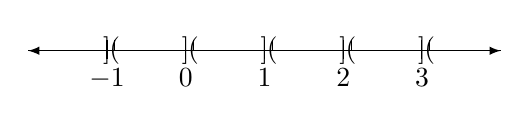
\begin{tikzpicture}
				\draw[latex-] (-2, 0) -- (4, 0);
				\draw[-latex] (-2, 0) -- (4, 0);
				
				% lines on numberline
				\foreach \x in {-1, 0, 1, 2, 3}
				\draw[shift={(\x, 0)}, color=black] (0pt, 3pt) -- (0pt, -3pt);
				
				%numbers on numberline
				\foreach \x in {-1, 0, 1, 2, 3}
				\draw[shift={(\x, 0)}, color=black] (0pt, 0pt) -- (0pt, -3pt) node[below] {$\x$};
				
				\foreach \x in {-0.9, 0.1, 1.1, 2.1, 3.1}
				\draw[shift={(\x, 0)}, color=black] (0pt, 4pt) -- (0pt, 0pt) node {{}(};
				\foreach \x in {-1, 0, 1, 2, 3}
				\draw[shift={(\x, 0)}, color=black] (0pt, 4pt) -- (0pt, 0pt) node {{}]};
			\end{tikzpicture}
		\end{figure}
		\item $\underset{n \in \mathbb{Z}}{\cup} (n, n+1 ] = \mathbb{R}$
		\item $(n, n+1 ] \cap (m, m+1 ] = \emptyset$ if $n \neq m$
		\item[Definition:] If $R$ is an equivalence relations on a set $A$ and $x \in A$, the equivalence class of $x$ denoted $[x]_R$ is the set $\{y \mid xRy \}.$ The collection of all equivalence classes is called $A$ modulo $R$ and denoted $A/R$.
		\item[Examples:]
		\begin{enumerate}
			\item[]
			\item $A = \mathbb{N} \hspace{10mm} x \equiv y$ mod 3 \\
			We have the equivalence classes $[0]_R, [1]_R$ and $[2]_R$ given by the then possible remainders under division by 3. \\
			${[0]}_R = \{0, 3, 6, 9, ...\}$ \\
			${[1]}_R = \{1, 4, 7, 10, ...\}$ \\
			${[2]}_R = \{2, 5, 8, 11, ...\}$ \\
			Clearly ${[0]}_R \cup {[1]}_R \cup {[2]}_R = \mathbb{N}$ and they are mutually disjoint $\Rightarrow R$ gives a partition of $\mathbb{N}$.
			\item $ABC \sim A'B'C'$ \\
			$[ABC] = \{$The set of all triangles with angles of magnitude $\measuredangle{ABC}, \measuredangle{BAC}, \measuredangle{ACB} \}$ \\
			The union over the set of all $[ABC]$ is the set of all triangles and $[ABC] \cap [A'B'Ç'] = \emptyset$ if $ABC \neq ^* A'B'C'$ since it means these triangles have at least one angle that if difference.
			\item [$^*$] In the original notes, not $\sim$ is used (a tilde with a slash going through it) but I couldn't find this symbol in latex.
			\item $A = \mathbb{C} \hspace{10mm} x \cap y$ if $|x| = |y|$ \hspace{10mm} equivalence relation \\
			$[x] = \{y \in \mathbb{C} \mid |x|=|y| \} = [r]$ for $r \in [0, +\infty) \land (r \geq 0)$ \\
			\begin{figure}[h]
				\centering
				\caption*{circle of radius $|x|$}
				\begin{tikzpicture}
					\draw(3, 0) -- (-3, 0) node[left]{Real};
					\draw(0, -3) -- (0, 3) node[above]{Imaginary};
					\draw{(0, 0)circle(2)};
				\end{tikzpicture}
			\end{figure}
			\\
			$\underset{r \in [0, +\infty)}{\cup} [r] = \mathbb{C}$ \\
			$[r_1] \cap [r_2] \neq \emptyset$ if $r_1 \neq r_2$ since two distinct circles in $\mathbb{C} \simeq \mathbb{R}^2$ with empty intersection.
			\pagebreak
			\begin{figure}[h]
				\centering
				\caption*{circles $r_1 \land r_2$}
				\begin{tikzpicture}
				\draw(-3, 0) -- (3, 0);
				\draw(0, -3) -- (0, 3);
				\draw{(0, 0)circle(2)};
				\draw{(0, 0)circle(1)};
				\end{tikzpicture}
			\end{figure}
		\end{enumerate}
		\item[Theorem:] For any equivalence relation $R$ on a set $A$, its equivalence classes form a partition of $A$, \textbf{i.e.}
		\begin{enumerate}
			\item $\forall x \in A, \exists y \in A$ s.t. $x \in [y]$ (every element of $A$ sits somewhere)
			\item $xRy \Leftrightarrow [x]=[y]$ (all elements related by $R$ belong to the same equivalence class)
			\item $\lnot (xRy) \Leftrightarrow [x] \cap [y] = \emptyset$ (if two elements are not related by $R$, the they belong to disjoint equivalence classes)
		\end{enumerate}
		\item[Proof:]
		\begin{enumerate}
			\item[]
			\item Trivial. Let $y=x$. $x \in [x]$ because $R$ is an equivalence relation. Hence reflexive, so $xRx$ holds.
			\item We will prove $xRy \Leftrightarrow [x] \subseteq [y]$ and $[y] \subseteq [x]$ \\
			$\Rightarrow$ Fix $x \in A, [x] = \{z \in A \mid xRz \} \Rightarrow \forall y \in A$ s.t. $xRy, y \in [x]$. Furthermore, $[y] = \{w \in A \mid yRw \}$ \\
			$\Rightarrow \forall w \in [u], yRw$ but $xRy \Rightarrow xRw$ by transitivity. Therefore, $w \in [x]$. We have shown $[y] \subseteq [x]$. \\
			Since $R$ is an equivalence relation, it is also symmetric. \textbf{i.e.} $xRy \Leftrightarrow yRx$. So by the same argument with $x$ and $y$ swapped $yRx \Rightarrow [x] \subseteq [y]$. Thus $xRy \Rightarrow [x] = [y]$. \\
			$\Rightarrow [x]=[y] \Rightarrow y \in [x]$ but $[x] = \{y \in A \mid xRy \}$
			\item $\Rightarrow$ We will prove the contrapositive. Assume $[x] \cap [y] \neq \emptyset \Rightarrow \exists z \in [x] \cap [y]. z \in [x]$ means $xRy$, whereas $z \in [y]$ means $yRx \Leftrightarrow zRy$ by symmetric of $R$. We thus have $xRz$ and $zRy \Rightarrow xRy$ by transitivity of $R. xRy$ contradicts $\lnot(xRy)$ so indeed $\lnot(xRy) \Rightarrow [x] \cap [y] = \emptyset$ \\
			$\Leftarrow$ Once again we use the contrapositive. \\
			Assume $\lnot(\lnot(xRy)) \Leftrightarrow xRy$. By part (b) $xRy \Rightarrow [x] = [y] \Rightarrow [x] \cap [y] \neq \emptyset$ since $x \in [x]$ and $y \in [y]$, \textbf{i.e.} These equivalence classes are non empty. We have obtained the needed contradiction.
		\end{enumerate}
		\item[qed]
		\item[Q:] What partition does "=" impose on $\mathbb{R}$?
		\item[A:] $[x]=\{x\}$ since $E = \{(x, x) \mid x \in \mathbb{R} \}$ the diagonal. \\
		The one element equivalence class is the smallest equivalence class possible (by definition, an equivalence class cannot be empty as it contains x itself). We call such a partition the \underline{finest} possible partition.
		\item[Remark:] The theorem above shows how every equivalence relations partitions a set. It turns out every partition of a set can be used to define an equivalence relation: $xRy$ is $x$ nd $y$ belong to the same subset of the partition (check this is indeed an equivalence relations!). Therefore, there is a 1-1 correspondence between partitions and equivlence relations: to each equivalence relation there corresponds a partition and vice versa.
	\end{description}
\end{document}